Distancia entre dos puntos equivalentes consecutivos en un onda. Puede ser entre crestas, valles o puntos de corte con la posición de equiilibrio. Se representa con la letra griega lambda $\lambda$.

Es la distancia de una oscilación completa.

Se mide en unidades de longitud. El Sistema internacional utiliza metros $m$.

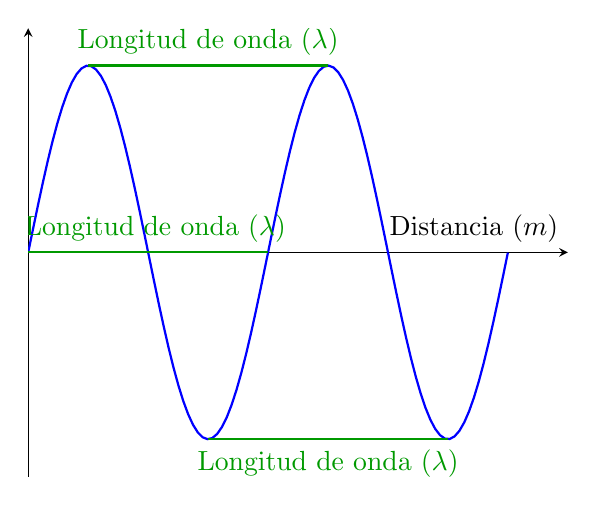
\begin{tikzpicture}
  \begin{axis}[
    xmin=0,xmax=4.5*pi,
    ymin=-1.2,ymax=1.2,
    axis lines=middle,
    xtick={0},
    ytick={0},
    xlabel=Distancia ($m$)
    ]

    % Funcion senoidal
    \addplot[color=blue,samples=100,domain=0:4*pi,thick]{sin(deg(x))};

    % Longitud de onda
    \draw[green!60!black,thick] (axis cs:0,0) -- (axis cs:2*pi,0) node[pos=0.53,above] {Longitud de onda ($\lambda$)};
    \draw[green!60!black,thick] (axis cs:pi/2,1) -- (axis cs:5*pi/2,1) node[pos=0.5,above] {Longitud de onda ($\lambda$)};
    \draw[green!60!black,thick] (axis cs:3*pi/2,-1) -- (axis cs:7*pi/2,-1) node[pos=0.5,below] {Longitud de onda ($\lambda$)};
  \end{axis}
\end{tikzpicture}

Considerando la distancia en metros y el número de ciclos u oscilaciones, se puede calcular de la siguiente manera:

\[\boxed{
  \lambda = \dfrac{\text{distancia} (m)}{\text{número de ciclos}}
}\]
